% start preamble -------------------------------------------------------------
\documentclass{article}
\usepackage{amsmath, amsthm, amssymb, amsfonts}
\usepackage{thmtools}
\usepackage{graphicx}
\usepackage{setspace}
\usepackage{geometry}
\usepackage{float}
\usepackage{hyperref}
\usepackage[utf8]{inputenc}
\usepackage[english]{babel}
\usepackage{framed}
\usepackage[dvipsnames]{xcolor}
\usepackage{tcolorbox}
\usepackage{ dsfont }
\usepackage[math]{cellspace}
\usepackage{ upgreek }
\setlength\cellspacetoplimit{3pt}
\setlength\cellspacebottomlimit{3pt}
\colorlet{LightGray}{White!90!Periwinkle}
\colorlet{LightOrange}{Orange!15}
\colorlet{LightGreen}{Green!15}

\graphicspath{ {./pictures/} }

\newcommand{\HRule}[1]{\rule{\linewidth}{#1}}
\newcommand{\tab}{\qquad \qquad}
% end preamble -------------------------------------------------------------------

\begin{document}

% ------------------------------------------------------------------------------
% Cover Page and ToC
% ------------------------------------------------------------------------------

\title{ \normalsize \textsc{}
		\\ [2.0cm]
		\HRule{1.5pt} \\
		\LARGE \textbf{\uppercase{ Mathe 2 Hausübung Nr.12 }
        \HRule{2.0pt} \\ [0.6cm] \LARGE{ Sebastian Steitz, Hannes Albert } \vspace*{10\baselineskip}}
		}
\date{Juli 2023}
\author{\textbf{} \\
		Gruppe: 6 \\
		Tutor: Zidane Bührmann }

\maketitle
\setlength\leftskip{1cm}
\section*{H12.1}
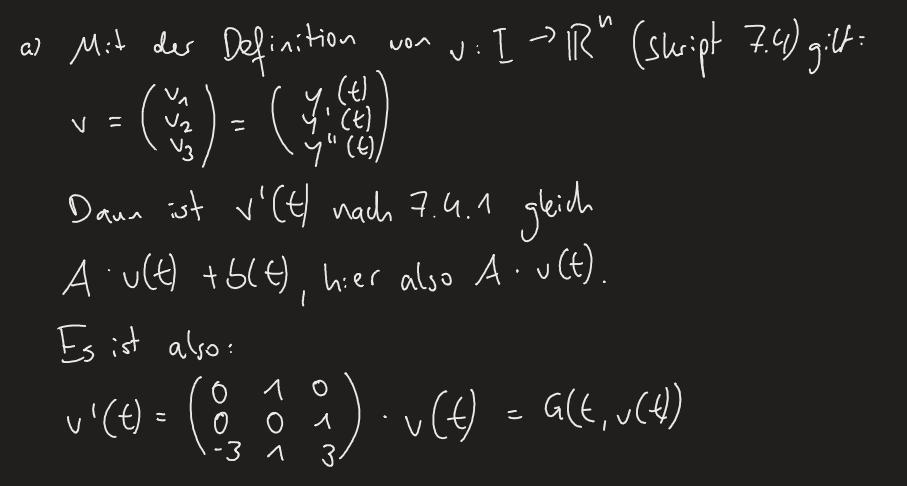
\includegraphics[scale=0.5]{1} \\
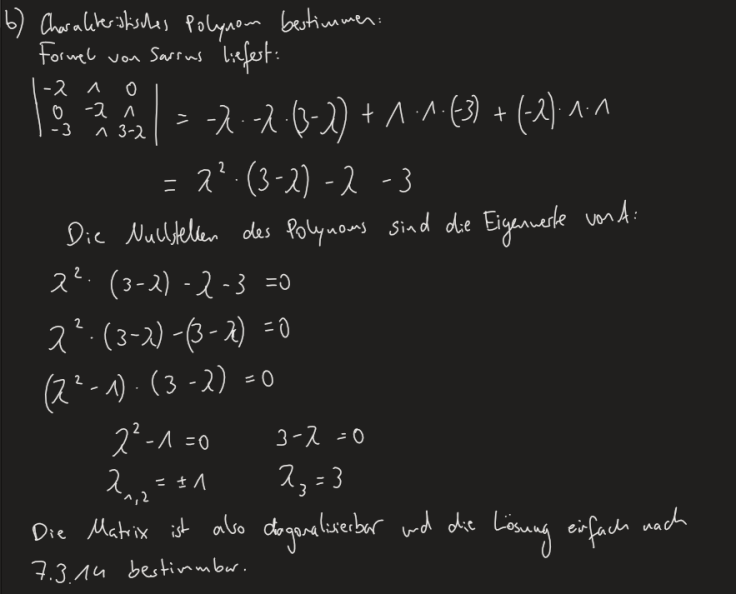
\includegraphics[scale=0.5]{2} \\ 
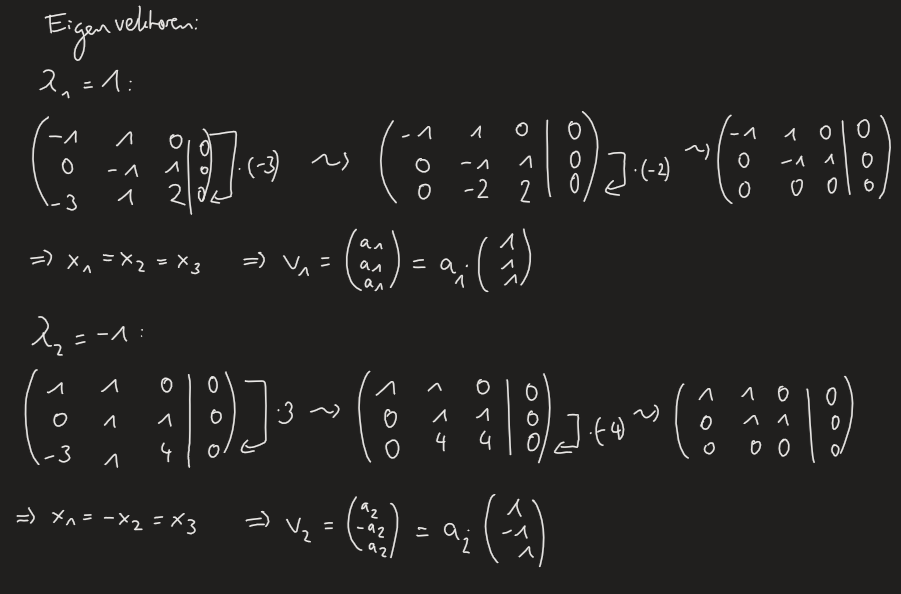
\includegraphics[scale=0.5]{3} \\ 
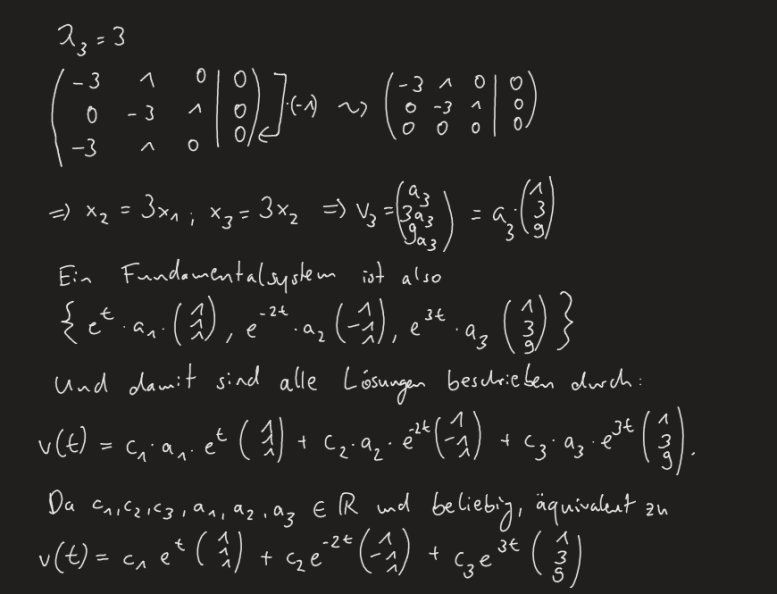
\includegraphics[scale=0.5]{4} \\ 

\includegraphics[scale=0.5]{5}

\section*{H12.2}
\noindent a) \\
Das charakteristische Polynom ergibt sich nach Definition 7.5.4:
\begin{align*}
    P &= \uplambda^3 - 5 * \uplambda^2 + 8 \uplambda - 4 \\ 
      &= \uplambda^3 - 4 * \uplambda^2 - \uplambda^2 + 8 \uplambda - 4 \\ 
      &= \uplambda^3 - 4 * \uplambda^2 - \uplambda^2 + 4 \uplambda + 4 \uplambda - 4 \\ 
      &= -1 * (\uplambda^2 - 4 \uplambda + 4) + \uplambda^3 - 4 \uplambda^2 + 4 \uplambda \\
      &= -1 * (\uplambda^2 - 4 \uplambda + 4) + \uplambda * (\uplambda^2 - 4 \uplambda + 4) \\
      &= (\uplambda - 1) * (\uplambda^2 - 4 \uplambda + 4) \\   
      &= (\uplambda - 1) * (\uplambda - 2)^2  
\end{align*}
$\rightarrow$ $\uplambda_1$ = 1 und $\uplambda_2$ = 2 (doppelte Nullstelle) \\
Damit erhalten wir für das Fundamentalsystem: F = \{$e^t$, $e^{2t}$, $te^{2t}$ \}
\[
    y(t) = C_1 * e^t + C_2 * e^{2t}  + C_3 * t * e^{2t} \tab C_1, C_2, C_3 \in \mathds{R} 
\]

\noindent b) \\
\begin{align*}
    P &= \uplambda^5 + 2 \uplambda^4 + \uplambda^3 \\ 
      &= \uplambda^3 * (\uplambda^2 + 2\uplambda + 1) \\ 
      &SvNP: \\ 
      &\uplambda^3 = 0 \\ 
      &\rightarrow \uplambda_1 = 0 (dreifache Nullstelle) \\ 
      &\uplambda_{2/3} = \frac{-2 \pm \sqrt{4 - 4 * 1 * 1}}{2} \\ 
      &= -\frac{2}{2} \\ 
      &= -1 \tab \rightarrow \text{doppelte Nullstelle}
\end{align*}
Somit ergibt sich für das Fundamentalsystem: \\ 
F = $\{ e^{0t}, te^{0t}, t^2 e^{0t}, e^{-t}, te^{-t}\}$ = $\{ 1, t, t^2, e^{-t}, te^{-t}\}$
\[
    y(t) = C_1 + C_2 * t  + C_3 * t^2 + C_4 * e^{-t} + C_5 * te^{-t} \tab C_i \in \mathds{R} \text{ mit i } \in \{1, 2, ... , 5\}
\]

\noindent c)
\begin{align*}
    P &= \uplambda^3 - \uplambda^2 + 2 * \uplambda - 2 \\ 
      &= (\uplambda^2 + 2) * (\uplambda - 1)
\end{align*}
$\rightarrow$ $\uplambda_1$ = $\sqrt{2}$i, $\uplambda_2$ = -$\sqrt{2}$i, $\uplambda_3$ = 1 \\ 
Somit ergibt sich für das Fundamentalsystem: \\ 
F = $\{e^{0t} * cos(\sqrt{2}t), e^{0t} * sin(\sqrt{2}t), e^t\}$ = $\{cos(\sqrt{2}t), sin(\sqrt{2}t), e^t\}$
\[
    y(t) = cos(\sqrt{2}t) * C_1 +  sin(\sqrt{2}t) * C_2 +  e^t * C_3 \tab C_1, C_2, C_3 \in \mathds{R}
\]
\end{document}

